\documentclass[aspectratio=169]{beamer}

% Use the course slide style when it is available. The fallback lets this file
% compile as a standalone deck outside the main project folder.
\IfFileExists{../downey_format_slides.sty}{%
    \usepackage{../downey_format_slides}%
}{%
    \usepackage{graphicx}
    \usepackage{amsmath,amssymb,bm}
    \usepackage{tikz}
    \usepackage{booktabs}
    \usepackage{xcolor}
}

\usefonttheme{serif}
\setbeamercolor{normal text}{fg=black}
\setbeamercolor{structure}{fg=black}
\setbeamercolor{frametitle}{fg=black}
\setbeamercolor{caption name}{fg=black}
\setbeamercolor{caption}{fg=black}
\setbeamercolor{section in head/foot}{fg=black}
\setbeamercolor{title}{fg=black}

\usetheme{default}
\useoutertheme{default}
\useinnertheme{default}
\setbeamertemplate{navigation symbols}{}

\definecolor{myred}{RGB}{115,0,10}

\usepackage{color}
\newcommand{\bl}[1]{\textcolor[rgb]{0.00,0.00,1.00}{#1}}
\newcommand{\gr}[1]{\textcolor[rgb]{0.00,0.50,0.00}{#1}}
\newcommand{\rd}[1]{\textcolor[rgb]{0.75,0.00,0.00}{#1}}
\newcommand{\tl}[1]{\textcolor[rgb]{0,0.6,0.60}{#1}}

\usepackage{booktabs}
\usepackage{bm}
\usepackage{mdframed}
\usepackage{xcolor}
\usepackage{tikz}
\usetikzlibrary{arrows.meta,shapes.geometric,positioning}

% --- Custom footline ---
\setbeamertemplate{footline}{%
\leavevmode
\begin{beamercolorbox}[wd=\paperwidth,ht=0.1ex]{}
\color{myred}\rule{\paperwidth}{0.1ex}
\end{beamercolorbox}
\hbox{%
\begin{beamercolorbox}[wd=\paperwidth,ht=2.5ex,dp=1ex]{}
\hspace{1em}
\insertsection
\hfill
\insertframenumber{} / \inserttotalframenumber
\hspace{1em}
\end{beamercolorbox}%
}%
}
\setbeamertemplate{headline}{}
\setbeamerfont{footline}{size=\small}

% --- Figure helper ----------------------------------------------------------
% First tries the project figure folder. If those files are unavailable, it
% falls back to the extracted assets that are included with the downloadable zip.
\newcommand{\MissingGraphic}[1]{%
\fbox{\begin{minipage}[c][0.42\textheight][c]{0.86\linewidth}
\centering Missing figure:\\[0.4em]\texttt{\detokenize{#1}}
\end{minipage}}%
}

\newcommand{\MaybeGraphic}[2][]{%
\IfFileExists{../figures/#2.pdf}{\includegraphics[#1]{../figures/#2.pdf}}{%
\IfFileExists{../figures/#2.png}{\includegraphics[#1]{../figures/#2.png}}{%
\IfFileExists{../figures/#2.jpg}{\includegraphics[#1]{../figures/#2.jpg}}{%
\IfFileExists{../figures/#2.jpeg}{\includegraphics[#1]{../figures/#2.jpeg}}{%
\IfFileExists{ch8_slide_assets/#2.png}{\includegraphics[#1]{ch8_slide_assets/#2.png}}{%
\IfFileExists{ch8_slide_assets/#2.jpg}{\includegraphics[#1]{ch8_slide_assets/#2.jpg}}{\MissingGraphic{#2}}}}}}}%
}

\title{Chapter~8~Clustering}
\author{Austin R.J. Downey}
\date{}

\begin{document}

\section{Machine Learning for Engineering Problem Solving}
\frame{\titlepage}

\section{Chapter~8~Clustering}

%------------------------------------------------

\begin{frame}{Clustering}
\begin{columns}[T,onlytextwidth]

\column{0.43\textwidth}

Clustering groups observations that ``look similar'' without using labels.

\vspace{0.6em}

Key idea:
\begin{itemize}
\item No target vector \(\mathbf{y}\)
\item The algorithm discovers structure
\item Similar points are grouped together
\end{itemize}

\vspace{0.6em}

Useful when you:
\begin{itemize}
\item have no ground-truth labels
\item suspect hidden sub-populations
\item want exploratory structure
\end{itemize}

\column{0.55\textwidth}
\centering
\MaybeGraphic[width=\textwidth]{Clustering_vs_Classification}

\vspace{0.3em}
Classification uses labels; clustering does not.

\end{columns}
\end{frame}

%------------------------------------------------

\begin{frame}{Review: Wine Dataset}
\begin{columns}[T,onlytextwidth]

\column{0.40\textwidth}

The wine dataset contains:
\begin{itemize}
\item 178 wine samples
\item 3 known cultivars
\item 13 continuous measurements
\end{itemize}

\vspace{0.6em}

Examples of features:
\begin{itemize}
\item alcohol
\item flavonoids
\item magnesium
\item color intensity
\end{itemize}

\vspace{0.6em}

The labels are useful for checking results, but clustering does not use them.

\column{0.58\textwidth}
\centering
\MaybeGraphic[width=\textwidth]{wine_data_feature-feature}

\vspace{0.3em}
Feature-feature plots for the wine data.

\end{columns}
\end{frame}

%------------------------------------------------

\begin{frame}{What a Clustering Algorithm Sees}
\begin{columns}[T,onlytextwidth]

\column{0.45\textwidth}

The input is the feature matrix:

\[
X = \left[\mathbf{x}_1,\mathbf{x}_2,\ldots,\mathbf{x}_n\right]^T
\]

\vspace{0.4em}

Each observation is a feature vector:

\[
\mathbf{x}_i \in \mathbb{R}^d
\]

\vspace{0.5em}

There is no target vector \(\mathbf{y}\).

\column{0.52\textwidth}

Most clustering methods depend on a distance or similarity measure.

\vspace{0.5em}

A common choice is Euclidean distance:

\[
    d\left(\mathbf{x}_i,\mathbf{x}_j\right)
    =
    \left\lVert \mathbf{x}_i-\mathbf{x}_j \right\rVert_2
\]

\vspace{0.5em}

Feature scaling matters because large-range features can dominate this distance.

\[
\texttt{StandardScaler} \quad \text{is often a good default.}
\]

\end{columns}
\end{frame}

%------------------------------------------------

\begin{frame}{Different Methods Define ``Cluster'' Differently}
\begin{columns}[T,onlytextwidth]

\column{0.42\textwidth}

The main difference is the modeling assumption.

\vspace{0.5em}

\begin{itemize}
\item K-means: center-based clusters
\item Hierarchical: nested groups
\item DBSCAN/HDBSCAN: dense regions
\item Gaussian mixtures: probability distributions
\item Anomaly detection: low-likelihood points
\end{itemize}

\vspace{0.5em}

No single method is best for every dataset.

\column{0.56\textwidth}
\centering
\vspace{2em}

\includegraphics[width=\textwidth, trim={0cm 0cm 7.5cm 0cm}, clip]{../figures/Clustering_methods}

\includegraphics[width=0.68\textwidth, trim={11cm 0cm 0cm 0cm}, clip]{../figures/Clustering_methods} \\
\vspace{0.3em}
Common clustering ideas.

\end{columns}
\end{frame}

%------------------------------------------------

\section{K-Means}

\begin{frame}{K-Means}
\begin{columns}[T,onlytextwidth]

\column{0.42\textwidth}

K-means partitions data into a chosen number of clusters, \(k\).

\vspace{0.5em}

Each cluster is represented by a centroid.

\vspace{0.5em}

The algorithm assigns each observation to the nearest centroid.

\vspace{0.5em}



\column{0.56\textwidth}
\centering
\MaybeGraphic[width=\textwidth]{K-means_wine_data}

\vspace{0.3em}
Wine data using two standardized features.

\end{columns}
\end{frame}

%------------------------------------------------

\begin{frame}{Objective Function}
\begin{columns}[T,onlytextwidth]

\column{0.42\textwidth}

Given observations:

\[
X = \{\mathbf{x}_1,\mathbf{x}_2,\ldots,\mathbf{x}_n\}\subset \mathbb{R}^d
\]

K-means seeks:
\begin{itemize}
\item centroids \(\boldsymbol{\mu}_1,\ldots,\boldsymbol{\mu}_k\)
\item assignments \(c_i\in\{1,2,\ldots,k\}\)
\end{itemize}

\column{0.55\textwidth}

The objective is the within-cluster sum of squares:

\[
J = \sum_{i=1}^{n}
\left\lVert \mathbf{x}_i-\boldsymbol{\mu}_{c_i}\right\rVert^2
\]

\vspace{0.5em}

This is also called:
\[
\text{inertia}
\]

\vspace{0.5em}

Small \(J\) means points are close to their assigned centroids.

\vspace{0.4em}

The cluster label \(c_i\) is just an arbitrary index.

\end{columns}
\end{frame}

%------------------------------------------------

\begin{frame}{Assignment and Update Steps}
\begin{columns}[T,onlytextwidth]

\column{0.43\textwidth}

Lloyd's algorithm alternates between two steps.

\vspace{0.5em}

\textbf{1. Assignment step}

Assign each point to its closest centroid:

\[
    c_i = \arg\min_{j\in\{1,\ldots,k\}}
    \left\lVert \mathbf{x}_i-\boldsymbol{\mu}_j\right\rVert^2
\]

\column{0.53\textwidth}

\textbf{2. Update step}

Move each centroid to the mean of the points assigned to it:

\[
    \boldsymbol{\mu}_j
    =
    \frac{1}{|C_j|}
    \sum_{i:c_i=j}\mathbf{x}_i
\]

\vspace{0.5em}

Repeat until assignments stop changing or \(J\) changes very little.

\end{columns}
\end{frame}

%------------------------------------------------

\begin{frame}{Decision Regions}
\begin{columns}[T,onlytextwidth]

\column{0.38\textwidth}

The assignment step divides feature space into regions.

\vspace{0.5em}

Every point in a region is closest to the same centroid.

\vspace{0.5em}

These regions are also called:
\[
\text{Voronoi cells}
\]

\vspace{0.5em}

For K-means, the boundaries are determined by distance to centroids.

\column{0.60\textwidth}
\centering
\MaybeGraphic[width=\textwidth]{K-Means_decision_regions}

\vspace{0.3em}
K-means decision regions for \(k=3\).

\end{columns}
\end{frame}

%------------------------------------------------

\begin{frame}{Centroid Movement}
\begin{columns}[T,onlytextwidth]

\column{0.37\textwidth}

K-means starts from initial centroids.

\vspace{0.5em}

Then it repeatedly:
\begin{itemize}
\item assigns points
\item updates centroids
\item lowers or keeps the same objective value
\end{itemize}

\vspace{0.5em}

After several iterations, the centroids settle into stable positions.

\column{0.61\textwidth}
\centering
\MaybeGraphic[width=\textwidth]{K-means_centroid_updates}

\vspace{0.3em}
Centroid movement during Lloyd iterations.

\end{columns}
\end{frame}

%------------------------------------------------

\begin{frame}{Random Starts and Local Minima}
\begin{columns}[T,onlytextwidth]

\column{0.38\textwidth}

The K-means objective is not convex.

\vspace{0.5em}

Different initial centroids can lead to different final clusters.

\vspace{0.5em}

Practical fixes:
\begin{itemize}
\item run K-means multiple times
\item keep the lowest-inertia solution
\item use \texttt{k-means++} initialization
\end{itemize}

\column{0.60\textwidth}
\centering
\MaybeGraphic[width=\textwidth]{K-Means_random_starts}

\vspace{0.3em}
Different random starts can converge to different solutions.

\end{columns}
\end{frame}

%------------------------------------------------

\begin{frame}{Choosing the Number of Clusters}
\begin{columns}[T,onlytextwidth]

\column{0.47\textwidth}

The number of clusters, \(k\), must be chosen before fitting K-means.

\vspace{0.5em}

If \(k\) is too small:
\begin{itemize}
\item distinct groups may be merged
\end{itemize}

If \(k\) is too large:
\begin{itemize}
\item one group may be split artificially
\end{itemize}

\vspace{0.5em}

Elbow rule:
\[
\Delta J(k)=J(k-1)-J(k)
\]

\column{0.50\textwidth}

Silhouette value for point \(i\):

\[
    s_i = \frac{b_i-a_i}{\max(a_i,b_i)}
\]

\vspace{0.5em}

Interpretation:
\begin{itemize}
\item near \(1\): well inside its cluster
\item near \(0\): near a boundary
\item negative: possibly assigned poorly
\end{itemize}

\end{columns}
\end{frame}

%------------------------------------------------

\begin{frame}{Cluster Diagnostics}
\begin{columns}[T,onlytextwidth]

\column{0.36\textwidth}

Adding more clusters usually decreases inertia.

\vspace{0.6em}

So we look for where the improvement begins to level off.

\vspace{0.6em}

For the two-feature wine example, the diagnostics support \(k=3\).

\column{0.62\textwidth}
\centering
\MaybeGraphic[width=\textwidth]{K-Means_cluster_diagnostics}

\vspace{0.3em}
Inertia and mean silhouette score for different values of \(k\).

\end{columns}
\end{frame}

%------------------------------------------------

\begin{frame}{Practical Notes}

\begin{columns}[T,onlytextwidth]

\column{0.48\textwidth}

K-means is usually efficient.

\[
O(nkd)
\]

\vspace{0.4em}

where:
\begin{itemize}
\item \(n\): observations
\item \(k\): clusters
\item \(d\): features
\end{itemize}

\column{0.48\textwidth}

Practical defaults:
\begin{itemize}
\item scale continuous features
\item use multiple random starts
\item use \texttt{k-means++}
\item interpret clusters as distance-based groups
\end{itemize}

\vspace{0.5em}

K-means is not a classifier; it simply groups nearby points.

\end{columns}
\end{frame}

%------------------------------------------------

\begin{frame}{K-Means for Image Segmentation}
\begin{columns}[T,onlytextwidth]

\column{0.38\textwidth}

K-means can cluster pixels.

\vspace{0.5em}

For a color image, each pixel can be represented by:

\[
\mathbf{x}_i = \begin{bmatrix} R_i & G_i & B_i \end{bmatrix}^T
\]

\vspace{0.5em}

Replacing each pixel by its centroid color gives a segmented or compressed image.

\column{0.60\textwidth}
\centering
\MaybeGraphic[width=\textwidth]{K-Means_Image_segmentation}

\vspace{0.3em}
Grouping pixels by similarity in color space.

\end{columns}
\end{frame}

%------------------------------------------------

\begin{frame}{Limitations of K-Means}

K-means works best when clusters are:
\begin{itemize}
\item compact
\item approximately spherical
\item similar in size
\item reasonably separated
\end{itemize}

\vspace{0.7em}

K-means can perform poorly when clusters are:
\begin{itemize}
\item curved or nested
\item elongated
\item strongly overlapping
\item very different in density
\item affected by outliers
\end{itemize}

\vspace{0.7em}

These are consequences of the centroid-and-distance assumption.

\end{frame}

%------------------------------------------------

\section{8.2~Hierarchical Agglomerative Clustering}

\begin{frame}{Hierarchical Agglomerative Clustering}
\begin{columns}[T,onlytextwidth]

\column{0.37\textwidth}

Hierarchical clustering builds a nested sequence of clusters.

\vspace{0.5em}

Agglomerative clustering is bottom-up:
\begin{itemize}
\item start with individual observations
\item merge nearby groups
\item continue until one cluster remains
\end{itemize}

\vspace{0.5em}

The result is a hierarchy, not just one fixed \(k\).

\column{0.61\textwidth}
\centering
\resizebox{0.98\textwidth}{!}{%
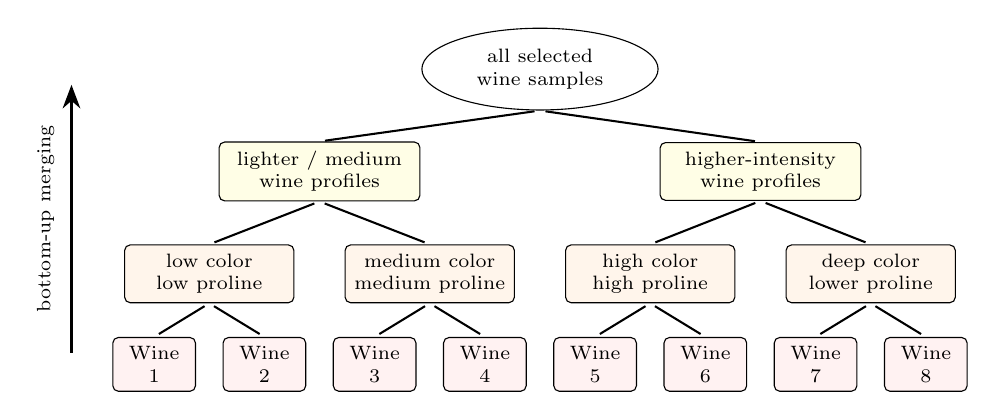
\begin{tikzpicture}[
    wine/.style={draw, rounded corners=2pt, fill=red!5, minimum width=1.05cm, minimum height=0.58cm, align=center, font=\scriptsize},
    cluster/.style={draw, rounded corners=2pt, fill=orange!8, minimum width=2.15cm, minimum height=0.68cm, align=center, font=\scriptsize},
    profile/.style={draw, rounded corners=2pt, fill=yellow!10, minimum width=2.55cm, minimum height=0.72cm, align=center, font=\scriptsize},
    root/.style={draw, ellipse, fill=white, minimum width=3.0cm, minimum height=0.72cm, align=center, font=\scriptsize},
    branch/.style={black, line width=0.75pt, shorten >=2pt, shorten <=2pt}
]
\node[wine] (w1) at (-4.9,0.0) {Wine\\1};
\node[wine] (w2) at (-3.5,0.0) {Wine\\2};
\node[wine] (w3) at (-2.1,0.0) {Wine\\3};
\node[wine] (w4) at (-0.7,0.0) {Wine\\4};
\node[wine] (w5) at (0.7,0.0)  {Wine\\5};
\node[wine] (w6) at (2.1,0.0)  {Wine\\6};
\node[wine] (w7) at (3.5,0.0)  {Wine\\7};
\node[wine] (w8) at (4.9,0.0)  {Wine\\8};
\node[cluster] (c12) at (-4.2,1.15) {low color\\low proline};
\node[cluster] (c34) at (-1.4,1.15) {medium color\\medium proline};
\node[cluster] (c56) at (1.4,1.15) {high color\\high proline};
\node[cluster] (c78) at (4.2,1.15) {deep color\\lower proline};
\node[profile] (c1234) at (-2.8,2.45) {lighter / medium\\wine profiles};
\node[profile] (c5678) at (2.8,2.45) {higher-intensity\\wine profiles};
\node[root] (all) at (0,3.75) {all selected\\wine samples};
\draw[branch] (w1.north) -- (c12.south);
\draw[branch] (w2.north) -- (c12.south);
\draw[branch] (w3.north) -- (c34.south);
\draw[branch] (w4.north) -- (c34.south);
\draw[branch] (w5.north) -- (c56.south);
\draw[branch] (w6.north) -- (c56.south);
\draw[branch] (w7.north) -- (c78.south);
\draw[branch] (w8.north) -- (c78.south);
\draw[branch] (c12.north) -- (c1234.south);
\draw[branch] (c34.north) -- (c1234.south);
\draw[branch] (c56.north) -- (c5678.south);
\draw[branch] (c78.north) -- (c5678.south);
\draw[branch] (c1234.north) -- (all.south);
\draw[branch] (c5678.north) -- (all.south);
\draw[-{Stealth[length=3mm]}, black, line width=0.8pt] (-5.95,0.15) -- (-5.95,3.55);
\node[rotate=90, font=\scriptsize] at (-6.28,1.85) {bottom-up merging};
\end{tikzpicture}%
}

\vspace{0.3em}
Representative bottom-up wine dendrogram.

\end{columns}
\end{frame}

%------------------------------------------------

\begin{frame}{Agglomerative Algorithm}

The basic algorithm is simple to state:

\vspace{0.4em}

\begin{enumerate}
\item Start with \(n\) clusters, one for each observation.
\item Compute distances between every pair of clusters.
\item Merge the two closest clusters.
\item Update distances to the new cluster.
\item Repeat until all observations have been merged into one cluster.
\end{enumerate}

\vspace{0.8em}

The key modeling decision is how to define the distance between two clusters.

\[
\text{distance between points} \quad \Longrightarrow \quad \text{distance between clusters}
\]

\end{frame}

%------------------------------------------------

\begin{frame}{Linkage Rules}
\begin{columns}[T,onlytextwidth]

\column{0.48\textwidth}

For clusters \(A\) and \(B\):

\vspace{0.4em}

\textbf{Single linkage}
\[
D_{\text{single}}(A,B)=
\min_{\mathbf{x}_i\in A,\mathbf{x}_j\in B}
    d(\mathbf{x}_i,\mathbf{x}_j)
\]

\textbf{Complete linkage}
\[
D_{\text{complete}}(A,B)=
\max_{\mathbf{x}_i\in A,\mathbf{x}_j\in B}
    d(\mathbf{x}_i,\mathbf{x}_j)
\]

\column{0.48\textwidth}

\textbf{Average linkage}
\[
D_{\text{average}}(A,B)=
\frac{1}{|A||B|}
\sum_{\mathbf{x}_i\in A}\sum_{\mathbf{x}_j\in B}
    d(\mathbf{x}_i,\mathbf{x}_j)
\]

\vspace{0.4em}

Interpretation:
\begin{itemize}
\item single: closest pair
\item complete: farthest pair
\item average: all pairwise distances
\end{itemize}

\end{columns}
\end{frame}

%------------------------------------------------

\begin{frame}{Ward Linkage}
\begin{columns}[T,onlytextwidth]

\column{0.47\textwidth}

Ward linkage merges the pair of clusters that causes the smallest increase in within-cluster variation.

\vspace{0.6em}

For cluster \(C\):

\[
W(C)=\sum_{\mathbf{x}_i\in C}
\left\lVert \mathbf{x}_i-\boldsymbol{\mu}_C\right\rVert^2
\]

\column{0.48\textwidth}

When clusters \(A\) and \(B\) are merged:

\[
\Delta W = W(A\cup B)-W(A)-W(B)
\]

\vspace{0.6em}

This is conceptually close to K-means because both methods favor compact clusters.

\end{columns}
\end{frame}

%------------------------------------------------

\begin{frame}{Dendrograms}

A dendrogram is a tree diagram showing the order in which clusters are merged.

\vspace{0.7em}

How to read it:
\begin{itemize}
\item bottom: individual observations
\item upward movement: clusters merge
\item merge height: dissimilarity between clusters
\item horizontal cut: produces a chosen clustering solution
\end{itemize}

\vspace{0.7em}

Why it is useful:
\begin{itemize}
\item inspect structure before choosing \(k\)
\item large vertical gaps suggest natural cuts
\item good for exploratory analysis and visualization
\end{itemize}

\vspace{0.7em}

Limitation: pairwise distances can make it expensive for large datasets.

\end{frame}

%------------------------------------------------

\section{8.3~Density-Based Methods}

\begin{frame}{Density-Based Methods: DBSCAN and HDBSCAN}
\begin{columns}[T,onlytextwidth]

\column{0.39\textwidth}

Density-based clustering defines clusters as dense regions separated by sparse regions.

\vspace{0.6em}

This is different from K-means:
\begin{itemize}
\item no centroid is needed
\item clusters can be curved
\item outliers can be labeled as noise
\end{itemize}

\vspace{0.6em}

The goal is to follow connected dense regions.

\column{0.59\textwidth}
\centering
\MaybeGraphic[width=\textwidth]{DBSCAN_vs_k-means}

\vspace{0.3em}
K-means versus DBSCAN on non-spherical data.

\end{columns}
\end{frame}

%------------------------------------------------

\begin{frame}{DBSCAN Parameters}
\begin{columns}[T,onlytextwidth]

\column{0.45\textwidth}

DBSCAN has two main parameters:

\vspace{0.5em}

\begin{itemize}
\item \(\epsilon\): neighborhood radius
\item \(\mathrm{minPts}\): minimum number of nearby points
\end{itemize}

\vspace{0.5em}

In scikit-learn:

\[
\mathrm{minPts} \quad \leftrightarrow \quad \texttt{min\_samples}
\]

\column{0.52\textwidth}

The \(\epsilon\)-neighborhood is:

\[
N_\epsilon(\mathbf{x}_i)=
\left\{
\mathbf{x}_j\in X:
    d(\mathbf{x}_i,\mathbf{x}_j)\leq \epsilon
\right\}
\]

A point is a core point if:

\[
\left|N_\epsilon(\mathbf{x}_i)\right|
\geq
\mathrm{minPts}
\]

\end{columns}
\end{frame}

%------------------------------------------------

\begin{frame}{Core, Border, and Noise Points}

DBSCAN separates observations into three roles.

\vspace{0.8em}

\begin{columns}[T,onlytextwidth]

\column{0.32\textwidth}
\textbf{Core point}
\begin{itemize}
\item dense neighborhood
\item at least \(\mathrm{minPts}\) points nearby
\item expands the cluster
\end{itemize}

\column{0.32\textwidth}
\textbf{Border point}
\begin{itemize}
\item not dense enough by itself
\item close to a core point
\item attached to a cluster
\end{itemize}

\column{0.32\textwidth}
\textbf{Noise point}
\begin{itemize}
\item not a core point
\item not close enough to a core point
\item remains unassigned
\end{itemize}

\end{columns}

\vspace{0.8em}

Clusters form by connecting chains of nearby core points.

\end{frame}

%------------------------------------------------

\begin{frame}{When \(\epsilon\) Is Too Small}
\begin{columns}[T,onlytextwidth]

\column{0.38\textwidth}

The choice of \(\epsilon\) sets the density scale.

\vspace{0.6em}

If \(\epsilon\) is too small:
\begin{itemize}
\item neighborhoods contain too few points
\item few points become core points
\item many observations become noise
\end{itemize}

\vspace{0.6em}

This does not mean the data have no structure; the density scale is wrong.

\column{0.60\textwidth}
\centering
\MaybeGraphic[height=0.68\textheight]{DBSCAN_eps_too_small}

\vspace{0.3em}
DBSCAN with \(\epsilon\) too small.

\end{columns}
\end{frame}

%------------------------------------------------

\begin{frame}{A More Useful \(\epsilon\)}
\begin{columns}[T,onlytextwidth]

\column{0.38\textwidth}

With a more useful \(\epsilon\):
\begin{itemize}
\item neighborhoods overlap
\item core points connect along the moons
\item two curved clusters are recovered
\item a few isolated points remain noise
\end{itemize}

\vspace{0.6em}

DBSCAN works well when clusters are connected dense regions.

\column{0.60\textwidth}
\centering
\MaybeGraphic[height=0.68\textheight]{DBSCAN_eps_neighborhoods}

\vspace{0.3em}
Overlapping neighborhoods connect core points.

\end{columns}
\end{frame}

%------------------------------------------------

\begin{frame}{Choosing \(\epsilon\) and Moving to HDBSCAN}
\begin{columns}[T,onlytextwidth]

\column{0.48\textwidth}

A common diagnostic is a nearest-neighbor distance plot.

\vspace{0.5em}

Procedure:
\begin{itemize}
\item compute distance to the \(k\)-th nearest neighbor
\item choose \(k\) near \(\mathrm{minPts}\)
\item sort distances from small to large
\item look for a sharp bend
\end{itemize}

\column{0.48\textwidth}

HDBSCAN reduces the need for one fixed \(\epsilon\).

\vspace{0.5em}

It builds a hierarchy over many density levels and keeps clusters that are stable.

\vspace{0.5em}

This helps when different clusters have different densities.

\end{columns}
\end{frame}

%------------------------------------------------

\begin{frame}{When to Use Density-Based Clustering}

Density-based clustering is a good choice when:

\vspace{0.5em}

\begin{itemize}
\item clusters may have irregular shapes
\item the data contain outliers
\item dense operating states are separated by sparse transitions
\item the number of clusters is not obvious
\end{itemize}

\vspace{0.8em}

DBSCAN is easiest to explain because \(\epsilon\) and \(\mathrm{minPts}\) have direct meanings.

\vspace{0.8em}

HDBSCAN is often more flexible when clusters have different densities.

\vspace{0.8em}

In both cases, feature scaling and the distance metric matter.

\end{frame}

%------------------------------------------------

\section{8.4~Gaussian Mixture Models}

\begin{frame}{Gaussian Mixture Models}
\begin{columns}[T,onlytextwidth]

\column{0.39\textwidth}

K-means assigns each observation to exactly one cluster.

\vspace{0.5em}

Gaussian mixture models provide a probabilistic alternative.

\vspace{0.5em}

The data are modeled as a weighted combination of Gaussian components.

\vspace{0.5em}

Overlap between components becomes membership uncertainty.

\column{0.59\textwidth}
\centering
\MaybeGraphic[width=\textwidth]{Gaussian_general_idea}

\vspace{0.3em}
One-dimensional GMM idea using wine color intensity.

\end{columns}
\end{frame}

%------------------------------------------------

\begin{frame}{Gaussian Mixture Density}
\begin{columns}[T,onlytextwidth]

\column{0.46\textwidth}

A Gaussian mixture model with \(k\) components has density:

\[
    p(\mathbf{x})
    =
    \sum_{j=1}^{k}
    \pi_j
    \mathcal{N}
    \left(
        \mathbf{x}
        \mid
        \boldsymbol{\mu}_j,
        \boldsymbol{\Sigma}_j
    \right)
\]

\column{0.50\textwidth}

The parameters are:
\begin{itemize}
\item \(\pi_j\): mixing weight
\item \(\boldsymbol{\mu}_j\): component mean
\item \(\boldsymbol{\Sigma}_j\): component covariance matrix
\end{itemize}

\vspace{0.5em}

The weights satisfy:
\[
\pi_j\geq 0,
\qquad
\sum_{j=1}^{k}\pi_j=1
\]

\vspace{0.3em}

\(\boldsymbol{\Sigma}_j\) controls each component's spread, shape, and orientation.

\end{columns}
\end{frame}

%------------------------------------------------

\begin{frame}{GMM Generative and Fitting Flow}
\centering
\resizebox{0.94\textwidth}{!}{%
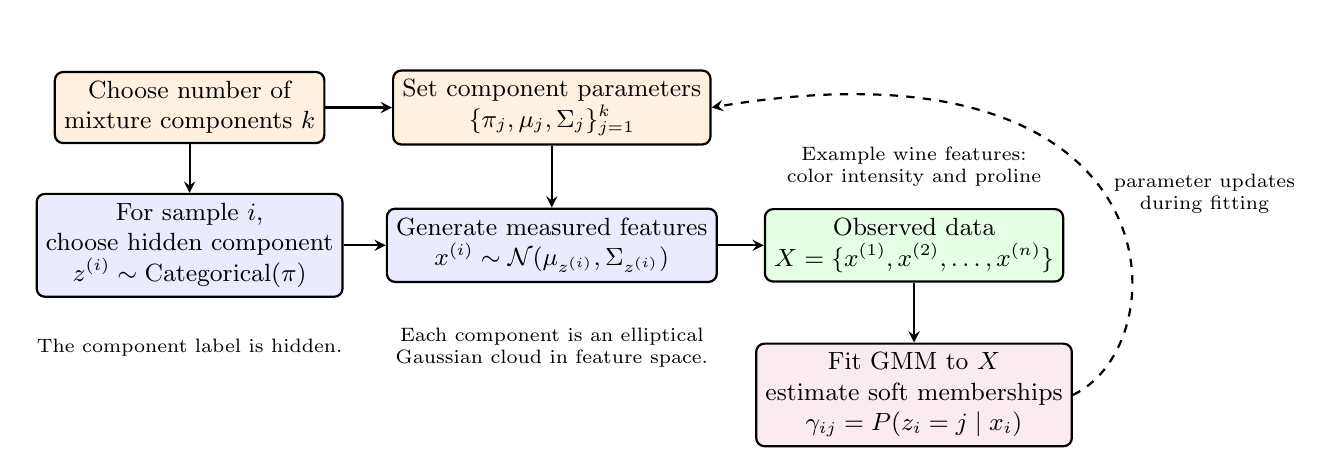
\begin{tikzpicture}[
    >=stealth,
    thick,
    process/.style={rectangle, draw, rounded corners=3pt, minimum width=3.35cm, minimum height=0.9cm, align=center, fill=blue!8},
    param/.style={rectangle, draw, rounded corners=3pt, minimum width=3.35cm, minimum height=0.9cm, align=center, fill=orange!12},
    data/.style={rectangle, draw, rounded corners=3pt, minimum width=3.35cm, minimum height=0.9cm, align=center, fill=green!10},
    output/.style={rectangle, draw, rounded corners=3pt, minimum width=3.35cm, minimum height=0.9cm, align=center, fill=purple!8},
    note/.style={align=center, font=\scriptsize},
    every node/.style={font=\small}
]
\node[param] (k) at (-4.6,2.0) {Choose number of\\mixture components \(k\)};
\node[param] (params) at (0,2.0) {Set component parameters\\\(\{\pi_j,\mu_j,\Sigma_j\}_{j=1}^{k}\)};
\node[process] (latent) at (-4.6,0.25) {For sample \(i\),\\choose hidden component\\\(z^{(i)} \sim \mathrm{Categorical}(\pi)\)};
\node[process] (sample) at (0,0.25) {Generate measured features\\\(x^{(i)} \sim \mathcal{N}\!\left(\mu_{z^{(i)}},\Sigma_{z^{(i)}}\right)\)};
\node[data] (observed) at (4.6,0.25) {Observed data\\\(X=\{x^{(1)},x^{(2)},\ldots,x^{(n)}\}\)};
\node[output] (fit) at (4.6,-1.65) {Fit GMM to \(X\)\\estimate soft memberships\\\(\gamma_{ij}=P(z_i=j\mid x_i)\)};
\draw[->] (k) -- (params);
\draw[->] (k) -- (latent);
\draw[->] (params) -- (sample);
\draw[->] (latent) -- (sample);
\draw[->] (sample) -- (observed);
\draw[->] (observed) -- (fit);
\draw[->, dashed]
    (fit.east)
    .. controls (8,-1) and (8,3)
    .. (params.east)
    node[pos=0.52, right, note] {parameter updates\\during fitting};
\node[note] at (-4.6,-1.05) {The component label is hidden.};
\node[note] at (0,-1.05) {Each component is an elliptical\\Gaussian cloud in feature space.};
\node[note] at (4.6,1.25) {Example wine features:\\color intensity and proline};
\end{tikzpicture}%
}

\vspace{0.4em}
The model estimates hidden component memberships and component parameters.

\end{frame}

%------------------------------------------------

\begin{frame}{Soft Cluster Assignments}
\begin{columns}[T,onlytextwidth]

\column{0.44\textwidth}

A GMM assigns probabilities, not just hard labels.

\vspace{0.5em}

The responsibility of component \(j\) for observation \(i\) is:

\scriptsize
\[
    \gamma_{ij}
    =
    P(z_i=j\mid \mathbf{x}_i)
    =
    \frac{
        \pi_j
        \mathcal{N}(\mathbf{x}_i\mid\boldsymbol{\mu}_j,\boldsymbol{\Sigma}_j)
    }
    {
        \sum_{\ell=1}^{k}
        \pi_\ell
        \mathcal{N}(\mathbf{x}_i\mid\boldsymbol{\mu}_\ell,\boldsymbol{\Sigma}_\ell)
    }
\]
\normalsize

\column{0.52\textwidth}

Responsibilities satisfy:

\[
0\leq \gamma_{ij}\leq 1,
\qquad
\sum_{j=1}^{k}\gamma_{ij}=1
\]

\vspace{0.5em}

A hard label can still be produced:

\[
\hat{z}_i=\arg\max_j \gamma_{ij}
\]

\vspace{0.5em}

But the probabilities tell us how uncertain that assignment is.

\end{columns}
\end{frame}

%------------------------------------------------

\begin{frame}{Gaussian Mixture Clustering}
\begin{columns}[T,onlytextwidth]

\column{0.36\textwidth}

The fitted GMM can be used to:
\begin{itemize}
\item assign each wine to its most likely component
\item estimate component probabilities
\item evaluate density or likelihood
\end{itemize}

\vspace{0.7em}

Soft assignments are especially useful when components overlap.

\column{0.62\textwidth}
\centering
\MaybeGraphic[width=\textwidth]{Gaussian_mixture_cluster}

\vspace{0.3em}
GMM clustering using color intensity and proline.

\end{columns}
\end{frame}

%------------------------------------------------

\begin{frame}{Expectation-Maximization}
\begin{columns}[T,onlytextwidth]

\column{0.48\textwidth}

GMM parameters are usually estimated using EM.

\vspace{0.5em}

The objective is to maximize the log-likelihood:

\scriptsize
\[
    \ell(\Theta)
    =
    \sum_{i=1}^{n}
    \log\left[
        \sum_{j=1}^{k}
        \pi_j
        \mathcal{N}
        (\mathbf{x}_i\mid\boldsymbol{\mu}_j,\boldsymbol{\Sigma}_j)
    \right]
\]
\normalsize

\column{0.48\textwidth}

EM alternates:

\vspace{0.5em}

\textbf{E-step}
\begin{itemize}
\item compute responsibilities \(\gamma_{ij}\)
\end{itemize}

\textbf{M-step}
\begin{itemize}
\item update weights, means, and covariances using weighted averages
\end{itemize}

\vspace{0.5em}

Repeat until the log-likelihood changes very little.

\end{columns}
\end{frame}

%------------------------------------------------

\begin{frame}{Covariance Structure}
\begin{columns}[T,onlytextwidth]

\column{0.38\textwidth}

The covariance matrix controls the shape and orientation of each component.

\vspace{0.5em}

Common choices:
\begin{itemize}
\item spherical: circular contours
\item diagonal: different variance by feature
\item tied: shared covariance
\item full: separate tilted ellipses
\end{itemize}

\column{0.60\textwidth}
\centering
\MaybeGraphic[width=\textwidth]{Gaussian_mixture_covariance}

\vspace{0.3em}
Different covariance assumptions on the wine data.

\end{columns}
\end{frame}

%------------------------------------------------

\begin{frame}{Choosing the Number of GMM Components}
\begin{columns}[T,onlytextwidth]

\column{0.48\textwidth}

GMMs also require choosing \(k\), the number of components.

\vspace{0.6em}

Because GMMs are probabilistic, likelihood-based criteria are common.

\vspace{0.6em}

They balance:
\begin{itemize}
\item model fit
\item model complexity
\end{itemize}

\column{0.48\textwidth}

Two common criteria:

\[
\mathrm{AIC}=2p-2\ell(\hat{\Theta})
\]

\[
\mathrm{BIC}=p\log(n)-2\ell(\hat{\Theta})
\]

\vspace{0.5em}

Lower values indicate a better tradeoff.

\vspace{0.3em}

BIC penalizes complexity more strongly when \(n\) is large.

\end{columns}
\end{frame}

%------------------------------------------------

\begin{frame}{Relationship Between K-Means and GMMs}

K-means can be viewed as a limiting case of a Gaussian mixture model.

\vspace{0.8em}

If all components have:
\begin{itemize}
\item spherical covariance matrices
\item equal variance
\item very small variance
\end{itemize}

then assigning a point to the most likely component becomes similar to assigning it to the nearest mean.

\vspace{0.8em}

So K-means is like a:
\[
\text{hard-assignment, equal-variance version of a GMM}
\]

\vspace{0.5em}

GMMs are more flexible, but they estimate more parameters.

\end{frame}

%------------------------------------------------

\section{8.5~Anomaly Detection}

\begin{frame}{Anomaly Detection}

Clustering methods can also help identify observations that do not fit any group well.

\vspace{0.8em}

These unusual observations may be called:
\begin{itemize}
\item anomalies
\item outliers
\item novelties
\end{itemize}

\vspace{0.8em}

In engineering, anomalies may correspond to:
\begin{itemize}
\item faulty sensors
\item rare operating conditions
\item damaged components
\item unusual loading events
\item data-entry errors
\end{itemize}

\end{frame}

%------------------------------------------------

\begin{frame}{Likelihood-Based Anomaly Detection}
\begin{columns}[T,onlytextwidth]

\column{0.48\textwidth}

A simple idea:
\begin{enumerate}
\item fit a model to normal data
\item evaluate likelihood for each observation
\item flag low-likelihood observations
\end{enumerate}

\vspace{0.6em}

For a Gaussian model:

\[
    p(\mathbf{x})=
    \mathcal{N}(\mathbf{x}\mid\boldsymbol{\mu},\boldsymbol{\Sigma})
\]

\column{0.48\textwidth}

Apply a threshold \(\tau\):

\[
\hat{y}(\mathbf{x})=
\begin{cases}
\text{anomaly}, & p(\mathbf{x})<\tau,\\
\text{normal}, & p(\mathbf{x})\geq \tau.
\end{cases}
\]

\vspace{0.5em}

Equivalently:

\[
\log p(\mathbf{x}) < \log\tau
\]

\end{columns}
\end{frame}

%------------------------------------------------

\begin{frame}{Mahalanobis Distance}
\begin{columns}[T,onlytextwidth]

\column{0.46\textwidth}

Gaussian anomaly detection is closely related to Mahalanobis distance:

\[
D_M(\mathbf{x})=
\sqrt{
(\mathbf{x}-\boldsymbol{\mu})^T
\boldsymbol{\Sigma}^{-1}
(\mathbf{x}-\boldsymbol{\mu})
}
\]

\column{0.50\textwidth}

This measures distance from the mean after accounting for covariance.

\vspace{0.6em}

Important idea:
\begin{itemize}
\item far along a high-variance direction may be normal
\item moderate distance along a low-variance direction may be unusual
\end{itemize}

\end{columns}
\end{frame}

%------------------------------------------------

\begin{frame}{GMM Anomaly Detection}
\begin{columns}[T,onlytextwidth]

\column{0.38\textwidth}

A GMM extends anomaly detection to data with multiple normal regimes.

\vspace{0.6em}

A point is normal if it has high likelihood under at least one component.

\vspace{0.6em}

A point is anomalous if it has low likelihood under the entire mixture.

\vspace{0.5em}

The threshold controls the tradeoff between false alarms and missed anomalies.

\column{0.60\textwidth}
\centering
\MaybeGraphic[width=\textwidth]{Gaussian_anomaly_detection}

\vspace{0.3em}
Low-likelihood wine observations marked as potential anomalies.

\end{columns}
\end{frame}

%------------------------------------------------

\begin{frame}{Chapter 8 Takeaways}

Different clustering methods answer the same question using different assumptions.

\vspace{0.8em}

\begin{center}
\begin{tabular}{lll}
\toprule
Method & Cluster idea & Watch out for \\
\midrule
K-means & centroid distance & scale, \(k\), spherical clusters \\
Hierarchical & nested merges & linkage and pairwise cost \\
DBSCAN/HDBSCAN & dense regions & density scale and metric \\
GMM & probability components & covariance, \(k\), initialization \\
Anomaly detection & low likelihood & threshold choice \\
\bottomrule
\end{tabular}
\end{center}

\vspace{0.8em}

The final engineering step is always interpretation: connect the discovered structure back to the system that produced the data.

\end{frame}

%------------------------------------------------

\end{document}
